\documentclass[a4paper,11pt]{article}
\input{/home/tof/Documents/Cozy/latex-include/preambule_lua.tex}
\newcommand{\showprof}{show them}  % comment this line if you don't want to see todo environment
\fancyhead[L]{Collection de bandes dessinées}
\newdate{madate}{10}{09}{2020}
%\fancyhead[R]{\displaydate{madate}} %\today
%\fancyhead[R]{Seconde - SNT}
%\fancyhead[R]{Première - NSI}
\fancyhead[R]{Terminale - NSI}
\fancyfoot[L]{~\\Christophe Viroulaud}
\AtEndDocument{\label{lastpage}}
\fancyfoot[C]{\textbf{Page \thepage/\pageref{lastpage}}}
\fancyfoot[R]{\includegraphics[width=2cm,align=t]{/home/tof/Documents/Cozy/latex-include/cc.png}}

\begin{document}
\begin{Form}
\section{Problématique}
Le professeur possède une collection de bandes dessinées importantes et qu'il complète régulièrement. Une fois dans sa librairie préférée, il lui arrive de ne plus se souvenir où il en est exactement dans ses séries. De plus il prête régulièrement des livres à ces amis et aimerait pouvoir maintenir à jour l'état de ses étagères.
\begin{figure}[!h]
\centering
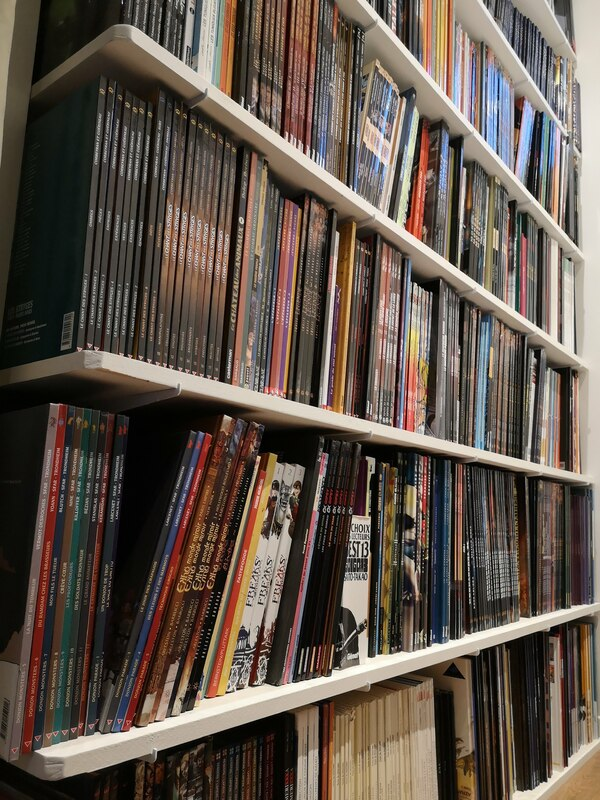
\includegraphics[width=3cm]{ressources/biblio.jpg}
\captionof{figure}{Bibliothèque}
\label{biblio}
\end{figure}

\begin{center}
\shadowbox{\parbox{17cm}{\centering Quelle solution peut-on mettre en place pour gérer efficacement la collection de bandes dessinées?}}
\end{center}
\section{Première approche}
La première approche imaginée consiste en l'utilisation d'un tableur (figure \ref{tableur}) pour stocker les informations.
\begin{figure}[!h]
\centering
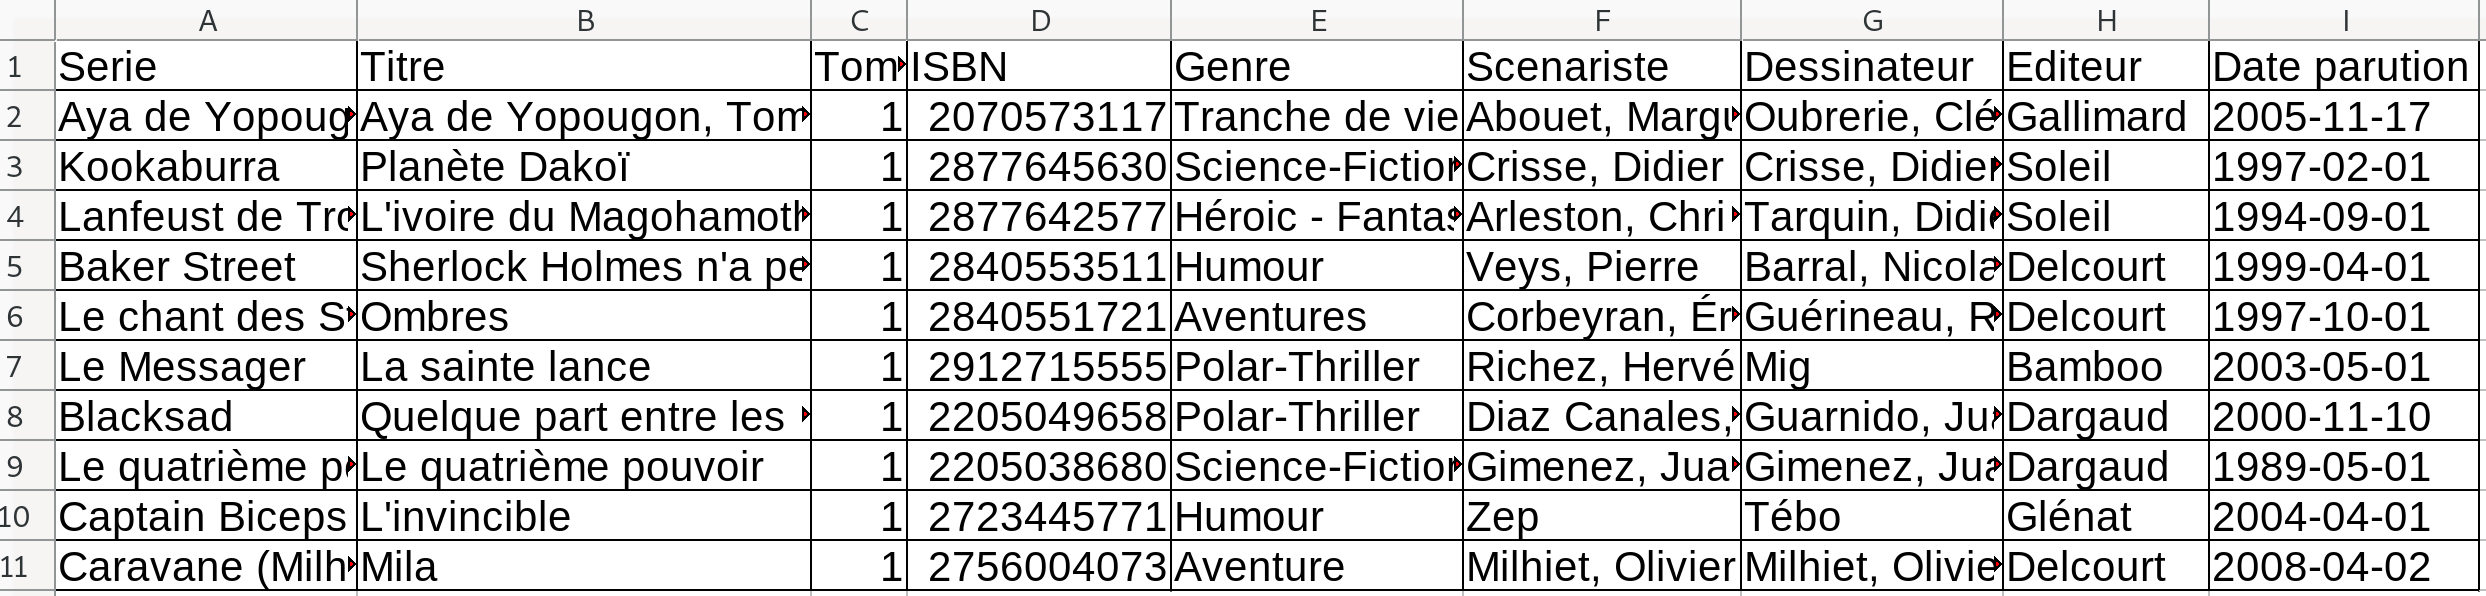
\includegraphics[width=15cm]{ressources/approche-1.png}
\captionof{figure}{Utilisation d'un tableur}
\label{tableur}
\end{figure}

Dans ce tableau, l'ajout d'une colonne \emph{emprunteur} permettrait de gérer les prêts.
\begin{activite}
Établir les limites de cette approche.
\end{activite}
\section{Modèle de données}
\subsection{Modèle relationnel}
La première étape est de définir la manière dont les données vont être représentées. Le \emph{modèle relationnel} est un des plus populaires. Dans ce modèle:
\begin{itemize}
\item Une \textbf{entité} (la bande dessinée) est un objet représenté par un n-uplet de valeurs scalaires.
\item Une \textbf{relation} (la collection) est l'ensemble des entités.
\end{itemize}
\begin{commentprof}
on peut s'arrêter à un csv mais:
\begin{itemize}
\item 2000 entrées = gérables par Python, mais si on veut étendre notre système à structure plus importante?
\item comment gérer modifications efficacement (ex: changement titre d'une série?)
\end{itemize}
scalaire = atomique
\subsection{Contexte historique}

\end{commentprof}

\end{Form}
\end{document}